\chapter{R\'esultats exp\'erimentaux}
\label{chap:resultats}

\section{Objectif et source de preuve}

Ce chapitre restitue le rapport d'\'evaluation promu avec les mod\`eles servis.
Toutes les valeurs proviennent du fichier \texttt{models/production/evaluation-report.json},
li\'e aux artefacts par sommes SHA-256. Le fichier source RT-IoT2022 contient
123\,117 lignes et 83 variables de mod\`ele. Son empreinte commence par
\texttt{956956c09c17}; elle correspond au manifeste de donn\'ees du projet.

\section{Qualit\'e, nettoyage et d\'es\'equilibre}

L'audit ne trouve aucune valeur manquante ou infinie. Il identifie toutefois six
signatures de variables associ\'ees \`a des labels contradictoires, soit 128 lignes.
Toutes ces lignes sont supprim\'ees afin de ne pas choisir arbitrairement un label.
Le nettoyage conserve ensuite un seul exemplaire de 5\,080 doublons de m\^eme label.

La distribution source est tr\`es d\'es\'equilibr\'ee: \texttt{DOS\_SYN\_Hping}
repr\'esente 94\,659 lignes, alors que \texttt{NMAP\_FIN\_SCAN} n'en contient que
28 et \texttt{Metasploit\_Brute\_Force\_SSH} 37. Pour cette raison, l'exactitude
globale n'est pas utilis\'ee seule; la macro-F1, le rappel par classe, le support et
le taux de faux positifs sont publi\'es.

L'analyse descriptive montre en outre des variables tr\`es asym\'etriques et de
nombreux z\'eros. Les graphiques emploient donc une transformation \texttt{log1p}
uniquement pour la visualisation. Les associations avec la cible restent
descriptives: elles peuvent r\'ev\'eler des artefacts de sc\'enario et ne sont pas
interpr\'et\'ees comme des causes d'attaque.

\section{Protocole exp\'erimental}

Apr\`es nettoyage, chaque graine (42, 1337 et 2026) produit un partage stratifi\'e
60\,/\,20\,/\,20 en entra\^inement, validation et test. Les indices sont communs
aux candidats d'une graine. Le pr\'etraitement et la calibration sigmo\"ide par
validation crois\'ee sont ajust\'es uniquement sur l'entra\^inement. La s\'election
maximise la macro-F1 moyenne de validation; le taux de faux positifs, la taille
s\'erialis\'ee et le nom stable d\'epartagent ensuite les candidats. Le test ne
participe jamais \`a ce choix.

Le fichier ne fournit aucun identifiant de session, d'appareil ou horodatage dont
la s\'emantique soit assez fiable pour construire un partage temporel ou group\'e.
Le protocole est donc une r\'ef\'erence interne r\'ep\'et\'ee, non une validation de
d\'eploiement.

\section{Comparaison des classifieurs}

\begin{table}[htbp]
  \centering
  \caption{Comparaison du d\'etecteur binaire sur les trois graines}
  \label{tab:binary-comparison}
  \renewcommand{\arraystretch}{1.15}
  \begin{tabular}{lrrrr}
    \toprule
    Mod\`ele & F1 validation & $\sigma$ & FPR validation & F1 test 42 \\
    \midrule
    R\'egression logistique & 0,9702 & 0,0028 & 5,5371\% & 0,9684 \\
    Arbre de d\'ecision & 0,9947 & 0,0006 & 0,7494\% & 0,9945 \\
    For\^et al\'eatoire & 0,9954 & 0,0006 & 0,9992\% & 0,9949 \\
    \textbf{Gradient boosting} & \textbf{0,9955} & 0,0003 & 0,8604\% & \textbf{0,9961} \\
    \bottomrule
  \end{tabular}
\end{table}

\begin{table}[htbp]
  \centering
  \caption{Comparaison du classifieur des familles d'attaque}
  \label{tab:multiclass-comparison}
  \renewcommand{\arraystretch}{1.15}
  \begin{tabular}{lrrrr}
    \toprule
    Mod\`ele & F1 validation & $\sigma$ & FPR macro & F1 test 42 \\
    \midrule
    R\'egression logistique & 0,6222 & 0,0745 & 0,2357\% & 0,6308 \\
    Arbre de d\'ecision & 0,9375 & 0,0060 & 0,0124\% & 0,9602 \\
    Gradient boosting & 0,9659 & 0,0070 & \textbf{0,0072\%} & 0,9619 \\
    \textbf{For\^et al\'eatoire} & \textbf{0,9668} & 0,0039 & 0,0104\% & \textbf{0,9642} \\
    \bottomrule
  \end{tabular}
\end{table}

Le gradient boosting est retenu pour la d\'etection et la for\^et al\'eatoire pour
les familles. Les \`ecarts de validation entre les meilleurs candidats sont
faibles; la r\`egle de s\'election d\'eclar\'ee, et non le score de test, d\'etermine
les champions. La figure~\ref{fig:notebook-comparison} montre la restitution
graphique g\'en\'er\'ee par le notebook ex\'ecutable.

\begin{figure}[htbp]
  \centering
  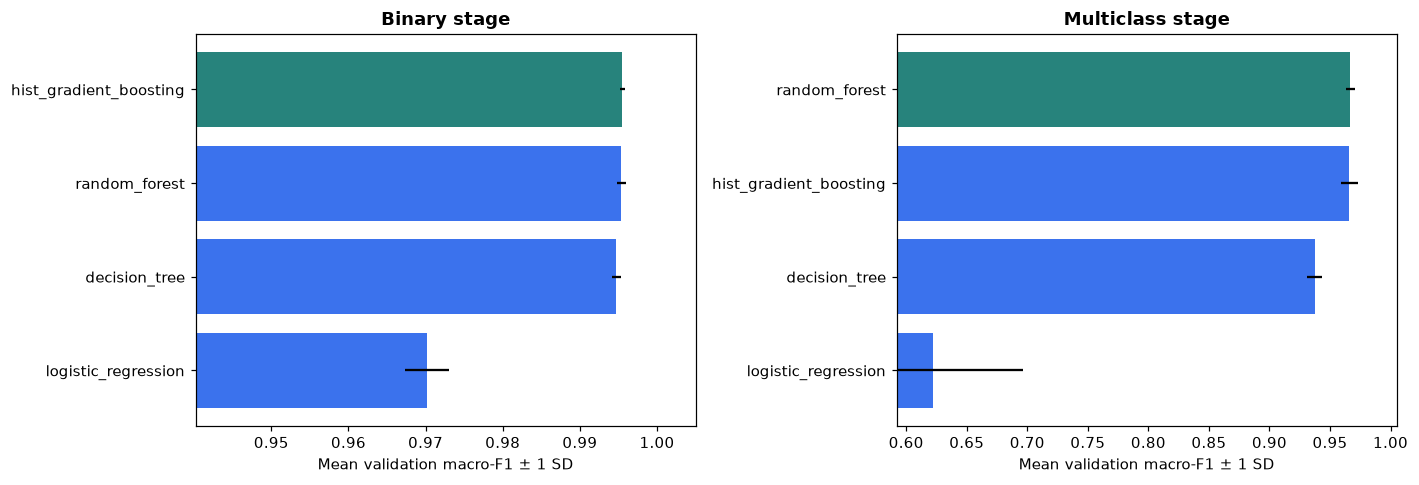
\includegraphics[width=0.92\textwidth,keepaspectratio]{assets/screenshots/notebook-model-comparison.png}
  \caption{Comparaison des candidats dans le notebook d'analyse}
  \label{fig:notebook-comparison}
\end{figure}

\section{Exp\'erience sur le d\'es\'equilibre}

Une exp\'erience diagnostique conserve l'architecture HistGradientBoosting et les
m\^emes partitions de la graine 42. Elle compare l'absence de correction, la
pond\'eration des classes et un sous-\'echantillonnage al\'eatoire limit\'e \`a
l'entra\^inement. Cette exp\'erience ne participe pas \`a la promotion.

\begin{table}[htbp]
  \centering
  \caption{Comparaison contr\^ol\'ee des traitements du d\'es\'equilibre}
  \label{tab:imbalance-comparison}
  \renewcommand{\arraystretch}{1.12}
  \begin{tabular}{llrrr}
    \toprule
    \`Etage & Traitement & Lignes fit & F1 validation & F1 test \\
    \midrule
    Binaire & Sans correction & 70\,745 & 0,9955 & 0,9969 \\
    Binaire & Pond\'eration & 70\,745 & 0,9946 & 0,9961 \\
    Binaire & Sous-\'echantillonnage & 14\,412 & 0,9891 & 0,9918 \\
    Familles & Sans correction & 63\,539 & 0,9528 & 0,9668 \\
    Familles & Pond\'eration & 63\,539 & 0,9368 & 0,9551 \\
    Familles & Sous-\'echantillonnage & 153 & 0,7150 & 0,7150 \\
    \bottomrule
  \end{tabular}
\end{table}

La pond\'eration am\'eliore l\'eg\`erement le rappel de la classe binaire minoritaire
(0,9975 contre 0,9946 sans correction), sans maximiser la macro-F1. Le
sous-\'echantillonnage conserve le support de la classe la plus rare pour chaque
classe et d\'etruit donc trop d'information, surtout au second \`etage o\`u seules
153 lignes subsistent. Cette comparaison montre qu'un r\'esultat agr\'eg\'e doit
toujours \^etre lu avec le rappel et le support des classes rares.

\section{Erreurs des champions et de la cascade}

La matrice binaire du test 42 contient 21\,159 attaques correctement d\'etect\'ees,
20 attaques manqu\'ees, 14 faux positifs et 2\,389 flux normaux correctement
reconnus. Le taux de faux positifs vaut ainsi 0,5826\%.

\begin{table}[htbp]
  \centering
  \caption{Classes les plus fragiles dans la cascade, graine 42}
  \label{tab:rare-errors}
  \begin{tabular}{lrrr}
    \toprule
    Classe & Support & Rappel & F1 \\
    \midrule
    NMAP\_FIN\_SCAN & 6 & 0,8333 & 0,7692 \\
    Metasploit\_Brute\_Force\_SSH & 7 & 0,7143 & 0,8333 \\
    DDOS\_Slowloris & 106 & 0,9528 & 0,9573 \\
    NMAP\_TCP\_scan & 200 & 0,9950 & 0,9975 \\
    \bottomrule
  \end{tabular}
\end{table}

La cascade compl\`ete atteint 0,9520 de macro-F1 pour la graine 42 et 0,9686 en
moyenne sur les trois graines. Le score 42 est sensible \`a une seule erreur parmi
six ou sept observations rares. Les supports sont donc indissociables des scores;
la valeur 0,9520 ne traduit pas une baisse uniforme sur les classes fr\'equentes.

\section{Calibration, seuil et co\^ut op\'erationnel}

Les deux champions sont calibr\'es par sigmoid sur l'entra\^inement. Sur le test
42, le d\'etecteur obtient un Brier de 0,0020 et une erreur de calibration attendue
de 0,0008; le classifieur obtient respectivement 0,0015 et 0,0010. Ces nombres ne
garantissent pas une calibration sur un autre r\'eseau. Le seuil de service 0,5 est
document\'e avec une courbe validation reliant faux positifs et attaques manqu\'ees.

Sur la machine de mesure, le p95 moyen par observation vaut 19,27~ms pour le
d\'etecteur et 31,79~ms pour le classifieur. Les artefacts occupent 418\,481 et
1\,325\,252 octets. Ces mesures comparent les candidats sur un h\^ote donn\'e et ne
constituent pas un objectif de capacit\'e en production.

\section{Menaces \`a la validit\'e}

Les r\'esultats restent internes \`a RT-IoT2022. Les classes rares rendent certaines
mesures instables; les doublons et artefacts de sc\'enario peuvent faciliter la
s\'eparation; aucune validation temporelle, par appareil, inter-r\'eseau ou
inter-jeu n'est disponible. La compatibilit\'e de noms avec un extracteur NFStream
ne prouve pas l'\'equivalence des valeurs. Enfin, la calibration et la latence sont
d\'ependantes du contexte de mesure. Ces limites interdisent de pr\'esenter le
prototype comme un contr\^ole de s\'ecurit\'e valid\'e sur un r\'eseau r\'eel.

\section{Conclusion}

L'exp\'erience r\'epond au cahier des charges: elle analyse les donn\'ees, compare
quatre mod\`eles, traite et mesure le d\'es\'equilibre, puis \`evalue les deux \`etages
et la cascade. Le meilleur r\'esultat reste une r\'ef\'erence reproductible interne;
une collecte autoris\'ee, group\'ee par session et s\'epar\'ee chronologiquement est
la prochaine preuve scientifique n\'ecessaire.
